%%%%%%%%%% EJERCICIO 2 %%%%%%%%%%

\begin{ejer}
    \textbf{Ejercicio 2. Un ejemplo clásico de red social de tamaño pequeño es el de las familias 
    más influyentes en la política, la economía y la vida social de la Florencia del siglo XV. 
    Los historiadores John Padgett y Christopher Ansell estudiaron esta red social en 1993, 
    basándose en datos tomados de archivos históricos (ver el artículo [2], que se ha adjuntado en 
    Recursos del aula virtual). El grafo que representa dicha red social, que no es dirigido, 
    y se forma dibujando una arista entre dos familias cada vez que un matrimonio las vincula, es el siguiente:}
\end{ejer}
 %%% IMAGEN DE FAMILIAS INFLUYENTES %%%
 \begin{figure}[H]
	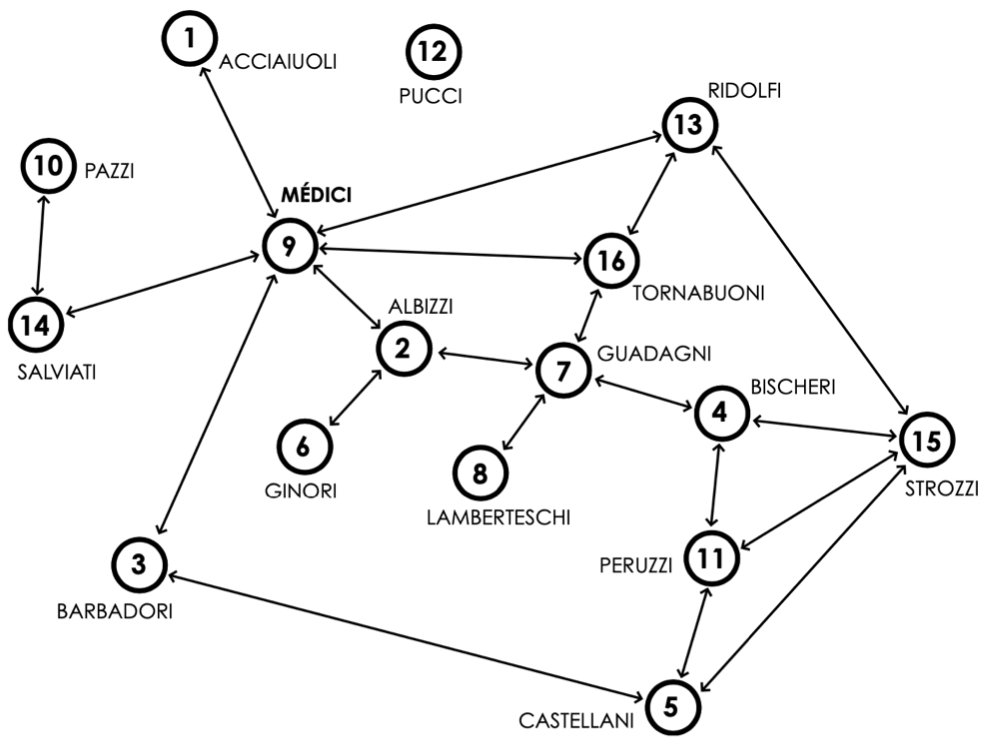
\includegraphics[width=\textwidth/2]{familiasInfluyentes}
	\centering
	\caption{Familias influyentes de Florencia.}
    \label{fig:familiasInfluyentes}
\end{figure}
\begin{ejer}
    \textbf{A simple vista se observa que la familia Médici, con el vértice $9$, ocupa una posición central, pues ostenta el grado máximo. 
    Los autores del estudio conjeturaron que los Médici alcanzaron una posición de dominio en la sociedad florentina precisamente forzando 
    su alianza con el resto de familias a través de múltiples matrimonios.}
\end{ejer}
\begin{ejer}
    \begin{itemize}
        \item \textbf{Aplica el algoritmo PageRank a esta red social para confirmar que, en efecto, la familia Médici era la más relevante en esta pequeña red social.}
    \end{itemize}
\end{ejer}

\begin{ejer}
    \begin{itemize}
        \item \textbf{Repite el apartado anterior, tomando ahora $p = 0$, $8ab$ y $p = 0$, $6ab$, donde $ab$ son las dos últimas cifras de tu DNI. ¿Varía mucho el resultado? ¿Por qué?}
    \end{itemize}
\end{ejer}

\begin{ejer}
    \begin{itemize}
        \item \textbf{Explica el resultado que has obtenido. ¿Qué se puede decir de las otras familias florentinas a partir de los datos obtenidos?}
    \end{itemize}
\end{ejer}